% Drawing 80/02-1 -- folder 80, batch 02, archive page 22 (PDF page 23).
% Transcription: à droite, un dessin : un faisceau de droites concourantes en un point, coupé par une droite transversale
% Kind: pencil of concurrent lines cut by a transversal. Method 2 (schematic redraw from the facsimile). Status: ok.
% Notes: Four lines through one point, cut by a long transversal below.
% Coordinates: 1 unit = 1 mm = 1/100 of the crop width (bbox in page fractions: [0.7, 0.15, 0.9, 0.21]).
% Redrawn by Claude (claude-opus-5-5), issue #73, 2026-11-07; not checked by a human; not compiled (no TeX in the session).
% Rights: reproduces part of the work -- behind RENDER_TRANSCRIPTS, never published by itself.
\documentclass[tikz,border=3pt]{standalone}
\usepackage{amsmath,amssymb}
\usetikzlibrary{patterns,arrows.meta}
\tikzset{pencil/.style={black!45}, struck/.style={black!35}, mark/.style={circle,draw,inner sep=1.3pt}, pt/.style={circle,fill,inner sep=0.9pt}, opt/.style={circle,draw,fill=white,inner sep=1.1pt}}
\begin{document}
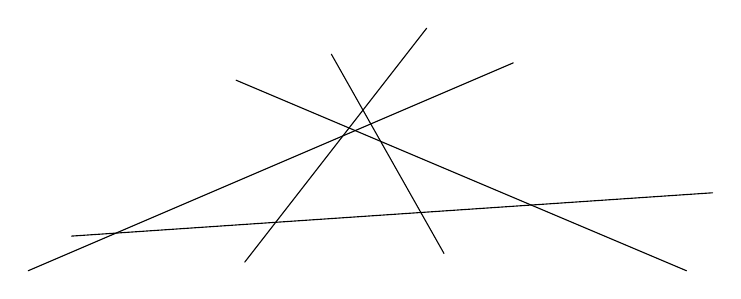
\begin{tikzpicture}[x=1mm,y=1mm,line cap=round,line join=round,font=\scriptsize]
\draw (5.5,-37.6) -- (67.1,-11.2);
\draw (44,-10.1) -- (58.3,-35.4);
\draw (31.9,-13.4) -- (89.1,-37.6);
\draw (33,-36.5) -- (56.1,-6.8);
\draw (11,-33.2) -- (92.4,-27.7);
\end{tikzpicture}
\end{document}
